%%%%%%%%%%%%%%%%%%%%%%%%%%%%%%%%%%%%%%%%%%%%%%%%%%%%%%%%%%%%
\documentclass[11pt]{article}
\usepackage[left=2cm,right=2cm,top=2cm,bottom=2cm]{geometry}
\usepackage{enumitem}
\usepackage{amsmath}
\usepackage{amsfonts}
\usepackage{amssymb}
\usepackage{amsthm}
\usepackage{verbatim}
\usepackage[capposition=top]{floatrow}
\numberwithin{equation}{section}
\usepackage[small,nohug,heads=vee]{diagrams}
\diagramstyle[labelstyle=\scriptstyle]
\usepackage{graphicx}
\DeclareGraphicsExtensions{.pdf,.eps,.jpg,.png}
\usepackage{subfig}
\usepackage[T1]{fontenc}
\usepackage{fmtcount}
\usepackage{longtable}
\usepackage[section]{placeins}
\newcommand{\HRule}{\rule{\linewidth}{1mm}}

% % % % % % % % % % % % % % % % % % % % % % %
%	Float rules rewritten
% See p.105 of "TeX Unbound" for suggested values.
    % See pp. 199-200 of Lamport's "LaTeX" book for details.
    %   General parameters, for ALL pages:
    \renewcommand{\topfraction}{0.9}	% max fraction of floats at top
    \renewcommand{\bottomfraction}{0.8}	% max fraction of floats at bottom
    %   Parameters for TEXT pages (not float pages):
    \setcounter{topnumber}{2}
    \setcounter{bottomnumber}{2}
    \setcounter{totalnumber}{2}     % 2 may work better
    \setcounter{dbltopnumber}{2}    % for 2-column pages
    \renewcommand{\dbltopfraction}{0.9}	% fit big float above 2-col. text
    \renewcommand{\textfraction}{0.07}	% allow minimal text w. figs
    %   Parameters for FLOAT pages (not text pages):
    \renewcommand{\floatpagefraction}{0.7}	% require fuller float pages
	% N.B.: floatpagefraction MUST be less than topfraction !!
    \renewcommand{\dblfloatpagefraction}{0.7}	% require fuller float pages

%%%%%%%%%%%%%%%%%%%%%%%%%%%%%%%%%%%%%%%%%%%%%%%%%%%%%%%%%%%%

\begin{document}

%%%%%%%%%%
%     TITLE PAGE     %
%%%%%%%%%%

\begin{titlepage}
\begin{center}

\includegraphics[natwidth = 700, natheight = 201, height = 3.5cm]{CarletonLogo.png}\\[0.5cm]    
\textsc{\large FACULTY OF SCIENCE - SCHOOL OF COMPUTER SCIENCE}\\[2cm]

\textsc{\Large PRINCIPLES OF COMPUTER NETWORKS}\\[0.2cm]
\textsc{\Large COMP 3203}\\[0.5cm]

\HRule \\[0.8cm]
{ \LARGE \bfseries DISCOVERY OF ROTATING DIRECTIONAL SENSORS}\\[0.5cm]
\HRule \\[1cm]

\Large
\emph{AUTHORS}\\[0.3cm]
\begin{center}
\begin{tabular}{lll}
Wesley \textsc{Lawrence} &Danil \textsc{Kirillov} &Darryl \textsc{Hill}\\
\end{tabular} 
\end{center}


\Large
\emph{PROFESSOR}\\[0.3cm]
Dr. Evangelos \textsc{Kranakis}\\[1cm]

{\large MONDAY, DECEMBER 3, 2012}

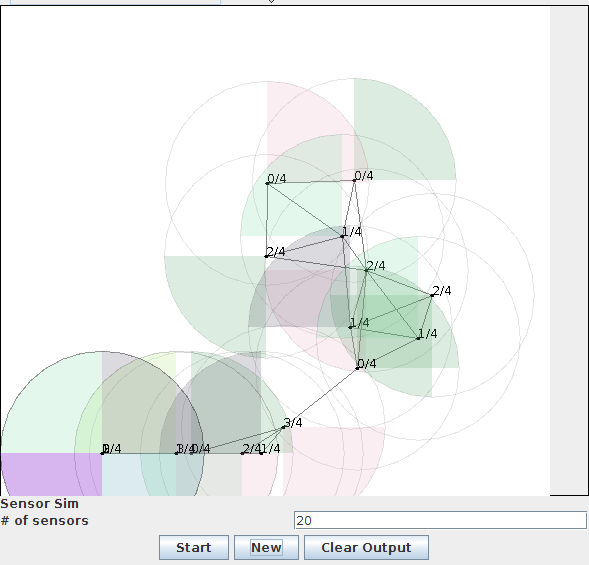
\includegraphics[height = 6cm]{pics/title.png}\\
\vfill


\end{center}
\end{titlepage}


%%%%%%%%%%%%%%
%     TABLE OF CONTENTS     %
%%%%%%%%%%%%%%

\newpage
\tableofcontents
\listoffigures

\section{Introduction}
In this document we examine the results of programmatically simulating algorithms for symmetry breaking for rotating directional sensors. We use the (D,D) model, whereby the sensors have identical transmission and reception beam width. Three algorithms are implemented.

\subsection{Antennae Rotation Algorithm}
In the ARA algorithm each sensor rotates one sector, then delays for $d_{u}$ steps while transmitting and listening for neighbours. In order to properly ensure that the sensors don't a)rotate with the same delay and b)rotate with delays that are multiples of one another, $d_{u}$ must be a prime number based on a colouring of the graph. 

\subsection{Random Selection Rotation Mechanism Algorithm}
In the RSRMA algorithm chooses between two algorithms, Mech0 and Mech1. Both take two arguments. Mech0 rotates with no sector delay, while Mech1 rotates using a sector delay. RSRMA calls these algorithms with the number of sectors as both arguments. So Mech0 rotates through its k sectors k times with no delay, while Mech1 rotates one sector then delays for k time while sending and listening for signals. At the end of each iteration it chooses Mech0 or Mech1 at random.

\subsection{Random Selection Rotation Mechanism Algorithm Prime}
RSRMA' operates much the same as RSRMA, except that instead of rotating through the k sectors k times in Mech0, or rotating through k sectors and delaying for k, it passes in a prime number (d) as the second argument. So it will rotate through the sectors d times in Mech0, or rotate with delay d in each sector in Mech1. At the end of each iteration it chooses Mech0 or Mech1 at random.
\section{Program Breakdown}

\subsection{MainThread}

The MainThread class is what really makes this application tick. As the name
suggest the class provides a thread on which the simulation is ran on. Prior to providing and running a thread, upon initialization, this class does a number of useful things. The first and foremost functionality it carries out is creating all
the Sensors. The number of sensors, as well as the number of sectors, and range is determined by parameters from the GUI, modified by the sliders. Creating Sensor
can be further broken down into three steps; deciding their placement, identifying the Neighbours, and assign the Sensor to and algorithm. <Something about
placement. Either a short description or something saying it's in another
section>.  Two Sensors are identified as Neighbours if both are in range of each other, falling on some sector of each other. Neighbours are identified in the
"record\_neighbours" method in the MainThread. This method is ran at most 
O(n$^{2}$)
times. Each call to this method passes in the index of a Sensor which needs to 
have it's Neighbours identified. The method then loops through all the Sensors up 
until the index passed in, so all the Sensors previously initialized. At each 
iteration of this loop, it checks if the Sensor at the current iteration of the 
loop is in range of the Sensor at the passed in index. If they are in range of 
each other, they are made Neighbours and a prime number is determined from the 168 
possible prime numbers for the Sensor at the passed in index, such that no 
neighbourly Sensors have the same prime number, thus effectively coloring the 
graph of Sensors both graph theory-wise and literally the Sensor's beam color. 
After the Neighbours are determined, each Sensor is assigned to an algorithm, this 
taking O(n) time, as it goes through each Sensor and assigns it to an algorithm. 
The type of algorithm that all the Sensors will be assigned to is determined by a 
parameter from the GUI. After the initialization the MainThread is prepared to 
run.  The run method of the MainThread, runs until the application is stopped and 
does one of the two things and is responsible for spawning the Java thread. It 
either re-initializes the Sensors if the user has pressed New. The main 
functionality that the run method provides is calling on update. In update the 
algorithms are updated, taking an O(n), where n is the amount of algorithms that 
have not yet been complete. An algorithm is complete when there are no remaining 
Neighbours for it's Sensor that need to be connected. Once the algorithm is 
complete it is then moved to another list, that acts an inactive list, so that it 
is on longer updated. This is to done to significantly improve the overall 
performance of the application, since the purpose of the simulation is to 
demonstrate how Sensors discover each other, once a Sensor has discovered all of 
it's neighbourly Sensors there is no need for it to keep searching/being updated. 
After the update has happened on the Algorithms, the Neighbours are checked for 
connection, followed by output to both the GUI and log, and a call to re-draw the 
sensors on the GUI. 

The current approach MainThread takes for "running" the sensors, is that there is a list of algorithms that are each responsible for "running" their Sensors. The algorithms themselves are all updating in the update method of the MainThread, and the MainThread is the only class responsible for spawning one thread that the repeatedly calls on update. The other approach would have been to allow each individual algorithm to spawn their own threads, which would then "run"/update the Sensors, while the MainThread handles checking Neighbour connects and calling on the GUI re-draw. During the development of this application, we have implemented this method. We've found that allowing each algorithm to have it's own separate thread would cause synchronization problems, would model a more practical simulation. However having just one thread in the MainThread and updating the algorithms in the update method that is repeatedly called on, the way that the runs application now, would model a more theoretical simulation, and thus this way was chosen to better demonstrate how the algorithms function and how the Sensors discover each other.
\section{Execution}


\section{Analysis}

\subsection{Comparison Methods}

Our main means of analysis was to compare algorithm performance over different numbers of sensors and different numbers of sectors. The number of sectors was the same for each sensor for each test, but could vary from test to test.

After building and testing the graphical environment, we set it up to execute batches of tests independant of the graphical interface. This allowed us to collect a lot of data quickly.

Specifically the batch runs would be for a particular number of sensors passed in as a command line argument. A second argument t is used for the number of tests to be run. The tests are run t times for each algorithm running over the k (number of sectors) values from 3 to 12. Log files are generated as well as statistical files. The statistical files are performance numbers formatted for graph generation. 
This data is then run through an averaging algorithm which reads in all the files, averages the individual tests while keeping the different sensor and sector values separate, and writes them out to another statistics file. This "average" statistics file is then used to generate a graph (a number of which are included in this write-up).

\subsection{Comparision}

As you can see in figures \ref{fig:n40k3}, \ref{fig:n40k7}, and \ref{fig:n40k12}, the highest performer at low numbers of sensors is RSRMA. If you remember, it passes in the number of sectors as its second argument and chooses between Mech0 and Mech1. The primary method of symmetry breaking of this algorithm is the random selection of either Mech0 or Mech1. Interestingly, for all the effort put into developing algorithms guaranteed to break symmetry, apparently sometimes it pays to simply roll the dice. 

You may also note that as the number of sectors decreases (ie the sector beam gets wider), ARA gets a noticable performance boost in comparison to the other two algorithms. 


\begin{figure}[ht]
\caption{}
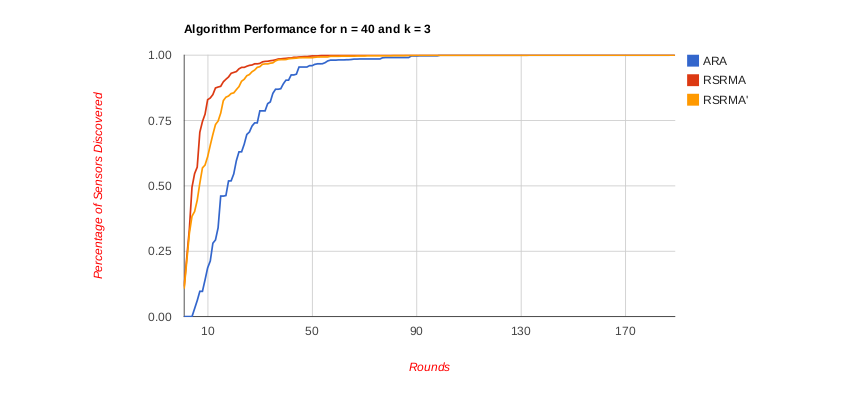
\includegraphics[height = 8cm]{pics/graph40k3.png}\\[0.5cm]    
\label{fig:n40k3}
\end{figure}

\begin{figure}[ht]
\caption{}
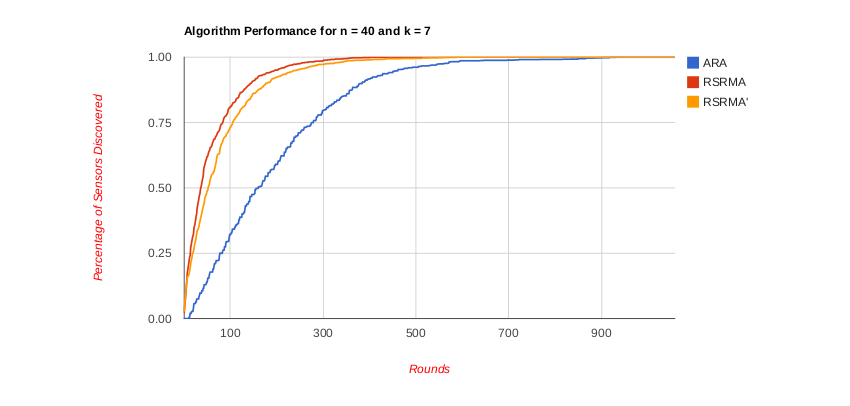
\includegraphics[height = 8cm]{pics/graph40k7.png}\\[0.5cm]   
\label{fig:n40k7} 
\end{figure}

\begin{figure}[ht]
\caption{}
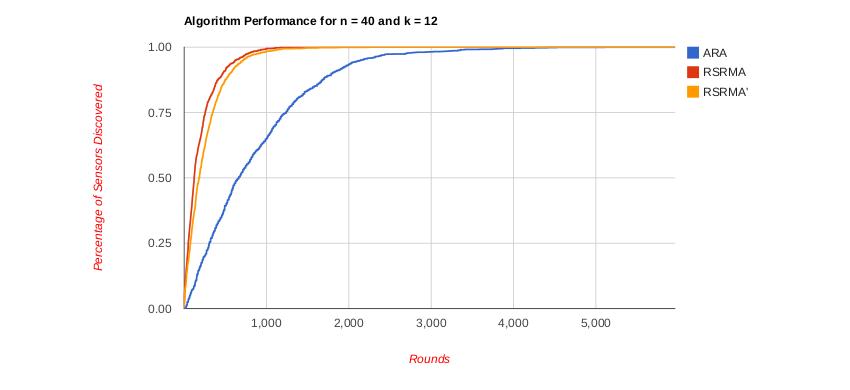
\includegraphics[height = 8cm]{pics/graph40k12.png}\\[0.5cm] 
\label{fig:n40k12}   
\end{figure}

At extremely low numbers of sensors, such as 10 (\ref{fig:n10k3}, \ref{fig:n10k7}, and \ref{fig:n10k12}) RSRMA and RSRMA' are difficult to distinguish. RSRMA starts out a bit quicker but by the end they are neck and neck. ARA is again the poor performer, but gets a boost at low k values.

\begin{figure}[ht]
\caption{}
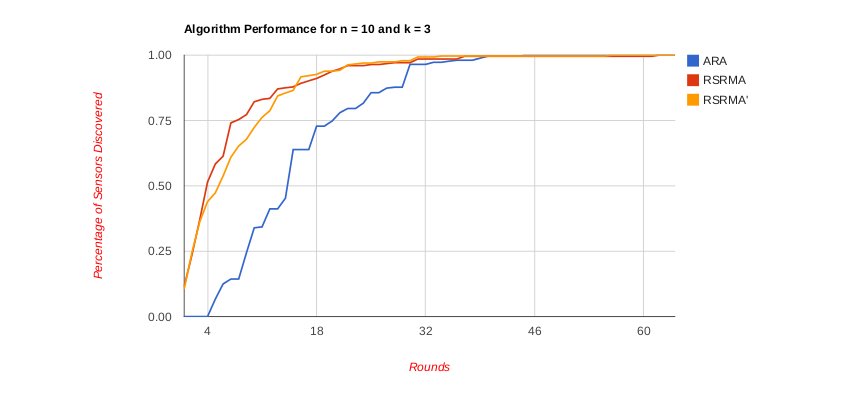
\includegraphics[height = 8cm]{pics/graph10k3.png}\\[0.5cm]    
\label{fig:n10k3}
\end{figure}

\begin{figure}[ht]
\caption{}
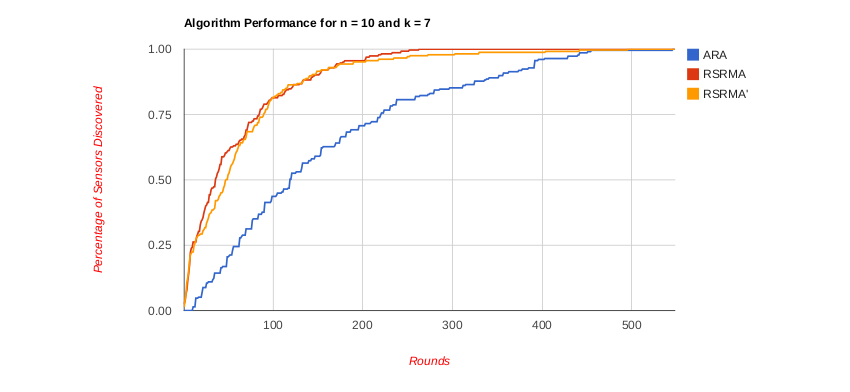
\includegraphics[height = 8cm]{pics/graph10k7.png}\\[0.5cm]   
\label{fig:n10k7} 
\end{figure}

\begin{figure}[ht]
\caption{}
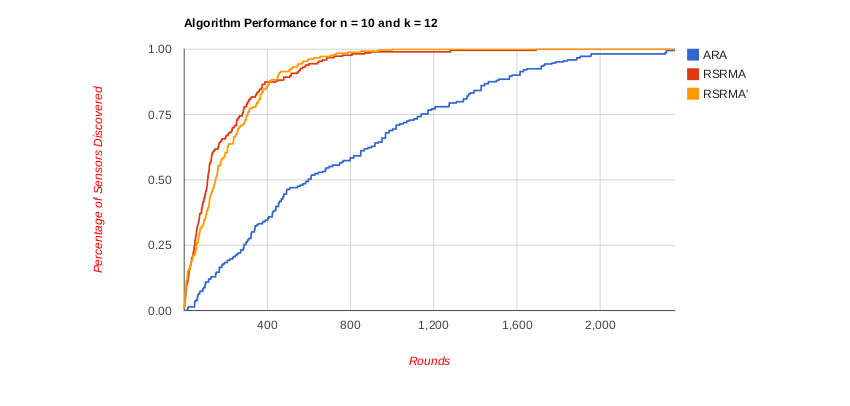
\includegraphics[height = 8cm]{pics/graph10k12.png}\\[0.5cm] 
\label{fig:n10k12}   
\end{figure}




%\section{Comparison Methods}
\section{Conclusions}

In overall algorithm performance, RSRMA is the clear winner. Not relying in global knowledge means it is versatile; it can be implemented anywhere, no just where there is global network knoweledge, and the overall simplicity of the algorithm provides another significant advantage. Moreover, its performance remains consistent even in dense graph situations, and/or with high k values. It is a solid performer in all areas and, relative to the other two algorithms implemented here, has no drawbacks.

ARA is purely deterministic. With a low number of sectors and a sparse graph it is a servicable algorithm. However, relying purely on prime numbers to break symmetry limits its usefulness in comparison to the other algorithms. In the situation of a high sector count (ie narrow sensor beam width) and/or a dense graph, we are forced to use higher and higher prime numbers to break symmetry, and the performance suffers. 

RSRMA' tries to combine the two approaches. It too suffers in dense graph situations or with high k values, due to high prime number cycles. In a combination of sparse graphs and low k values, where the prime numbers remain low, it is comparable to RSRMA. However, as the density and k value increase, the performance falls away. The randomized element means it does not suffer as much as ARA, and the determistic element guarantees completion. However in practice it is consistently outperformed by the purely random algorithm in high density and high k value scenarios.



\end{document}